%%%%%%%%%%%%%%%%%%%%%%%%%%%%%%%%%%%%%%%%%%%%%%%%%%%%%%%%%%%
%%%%%%%%%%%%%%%%%%%%%%%%%%%%%%%%%%%%%%%%%%%%%%%%%%%%%%%%%%%
\section{Parameter Identification and the MUD Point}
%%%%%%%%%%%%%%%%%%%%%%%%%%%%%%%%%%%%%%%%%%%%%%%%%%%%%%%%%%%
%%%%%%%%%%%%%%%%%%%%%%%%%%%%%%%%%%%%%%%%%%%%%%%%%%%%%%%%%%%

%%%%%%%%%%%%%%%%%%%%%%%%%%%%%%%%%%%%%%%%%%%%%%%%%%%%%%%%%%%
\begin{frame}[t]
\centering
\vskip 24pt
We formally define the maximal updated density (MUD) point as
\begin{equation}\label{eq:mudpt_inital_defn}
	\mudpt := \argmax {\updated}(\param).
\end{equation}

\vskip 24pt
We motivate the use of the MUD point as an alternative to the MAP point for parameter estimation problems.

\end{frame}

\begin{frame}[t]

Let $\norm{\mathbf{x}}_C^2 := (\mathbf{x}, \mathbf{x})_C = \mathbf{x}^T C \mathbf{x}$. \\

Inverse covariances associated with non-degenerative multivariate Gaussian distributions will play the role of $C$. \\

Suppose that the initial and prior densities are both given by the same $\mathcal{N}(\param_0, \initialCov)$ distribution.

\vskip 12pt
Additionally, suppose the map $Q$ is linear and that the data-likelihood and observed densities are both given by the same $\mathcal{N}(\observedMean, \observedCov)$ distribution.

\vskip 12pt
The linearity of $Q$ implies that $Q(\param)=A\param$ for some $A\in\RR^{d\times p}$, and that the predicted density follows a $\mathcal{N}(Q(\param_0), \predictedCov)$ distribution where
\begin{equation}\label{eq:predictCov}
	\predictedCov := A\initialCov A^\top.
\end{equation}

\end{frame}

%%%%%%%%%%%%%%%%%%%%%%%%%%%%%%%%%%%%%%%%%%%%%%%%%%%%%%%%%%
\subsection{Theory of Regularization}
%%%%%%%%%%%%%%%%%%%%%%%%%%%%%%%%%%%%%%%%%%%%%%%%%%%%%%%%%%

\begin{frame}[t]{\it The one with the regularization equations.}
%\vskip 25pt
\centering
\begin{figure}
\centering

\begin{table}[htbp]
\centering

\begin{tabular}{|c|c|}
\hline
  & \\
  $\displaystyle \updated(\param) = \initial(\param) \frac{\observed(Q(\param))}{\predicted(Q(\param))}$
&
  $\displaystyle \pi_{\text{post}}(\param\,|\,d) = \frac{\pi_{\text{prior}}(\param)\pi_\text{like}(d\,|\,\param)}{\int_{\Lambda} \pi_\text{like}(d\, |\, \param)  \pi_{\text{prior}}(\param) d\pmeas}$
\\
\hline
  & \\
  Tikhonov & $T(\param):=\norm{Q(\param)-\observedMean}_{\observedCov^{-1}}^2 +
      \norm{\param-\initialMean}_{\initialCov^{-1}}^2$
  \\ & \\ \hline & \\
  Data-Consistent & $J(\param):=T(\param) - \norm{Q(\param)-Q(\initialMean)}_{\predictedCov^{-1}}^2$
\\
& \\
  \hline
\end{tabular}
\caption{The $\param$ which minimizes these functionals also maximizes the updated PDF (left) and the Bayesian posterior PDF (right).

$T(\param)$ is the typical functional often associated with Tikhonov regularization.

The $J(\param)$ has an additional term subtracted from $T(\param)$ coming from the predicted density that serves as ``unregularization'' in data--informed directions.}
  \label{tab:func_comparisons}
\end{table}


\end{figure}

\end{frame}



%%%%%%%%%%%%%%%%%%%%%%%%%%%%%%%%%%%%%%%%%%%%%%%%%%%%%%%%%%%
\subsection{Linear Example}
%%%%%%%%%%%%%%%%%%%%%%%%%%%%%%%%%%%%%%%%%%%%%%%%%%%%%%%%%%%

%%%%%%%%%%%%%%%%%%%%%%%%%%%%%%%%%%%%%%%%%%%%%%%%%%%%%%%%%%%
\begin{frame}[t]{\it The one where an example highlights a key difference.}

\centering
Consider a linear QoI map is defined by $A=\mat{cc}{1 & 1}$. \\
2-D input, 1-D output $\implies$ rank-deficient

\vskip 12pt

Parameters in the initial and observed densities are given by
\begin{equation*}
\begin{split}
	\initialMean = \mat{cc}{0.25 & 0.25}^\top, \\
  \initialCov = \mat{cc}{1 & -0.25 \\ -0.25 & 0.5}, \\
  \observedMean=1, \text{ and } \observedCov = \mat{c}{0.25}
\end{split}
\end{equation*}

\end{frame}

%%%%%%%%%%%%%%%%%%%%%%%%%%%%%%%%%%%%%%%%%%%%%%%%%%%%%%%%%%%
\begin{frame}[t]
%\vskip 25pt
\centering
\begin{figure}
\centering

\begin{figure}
   % 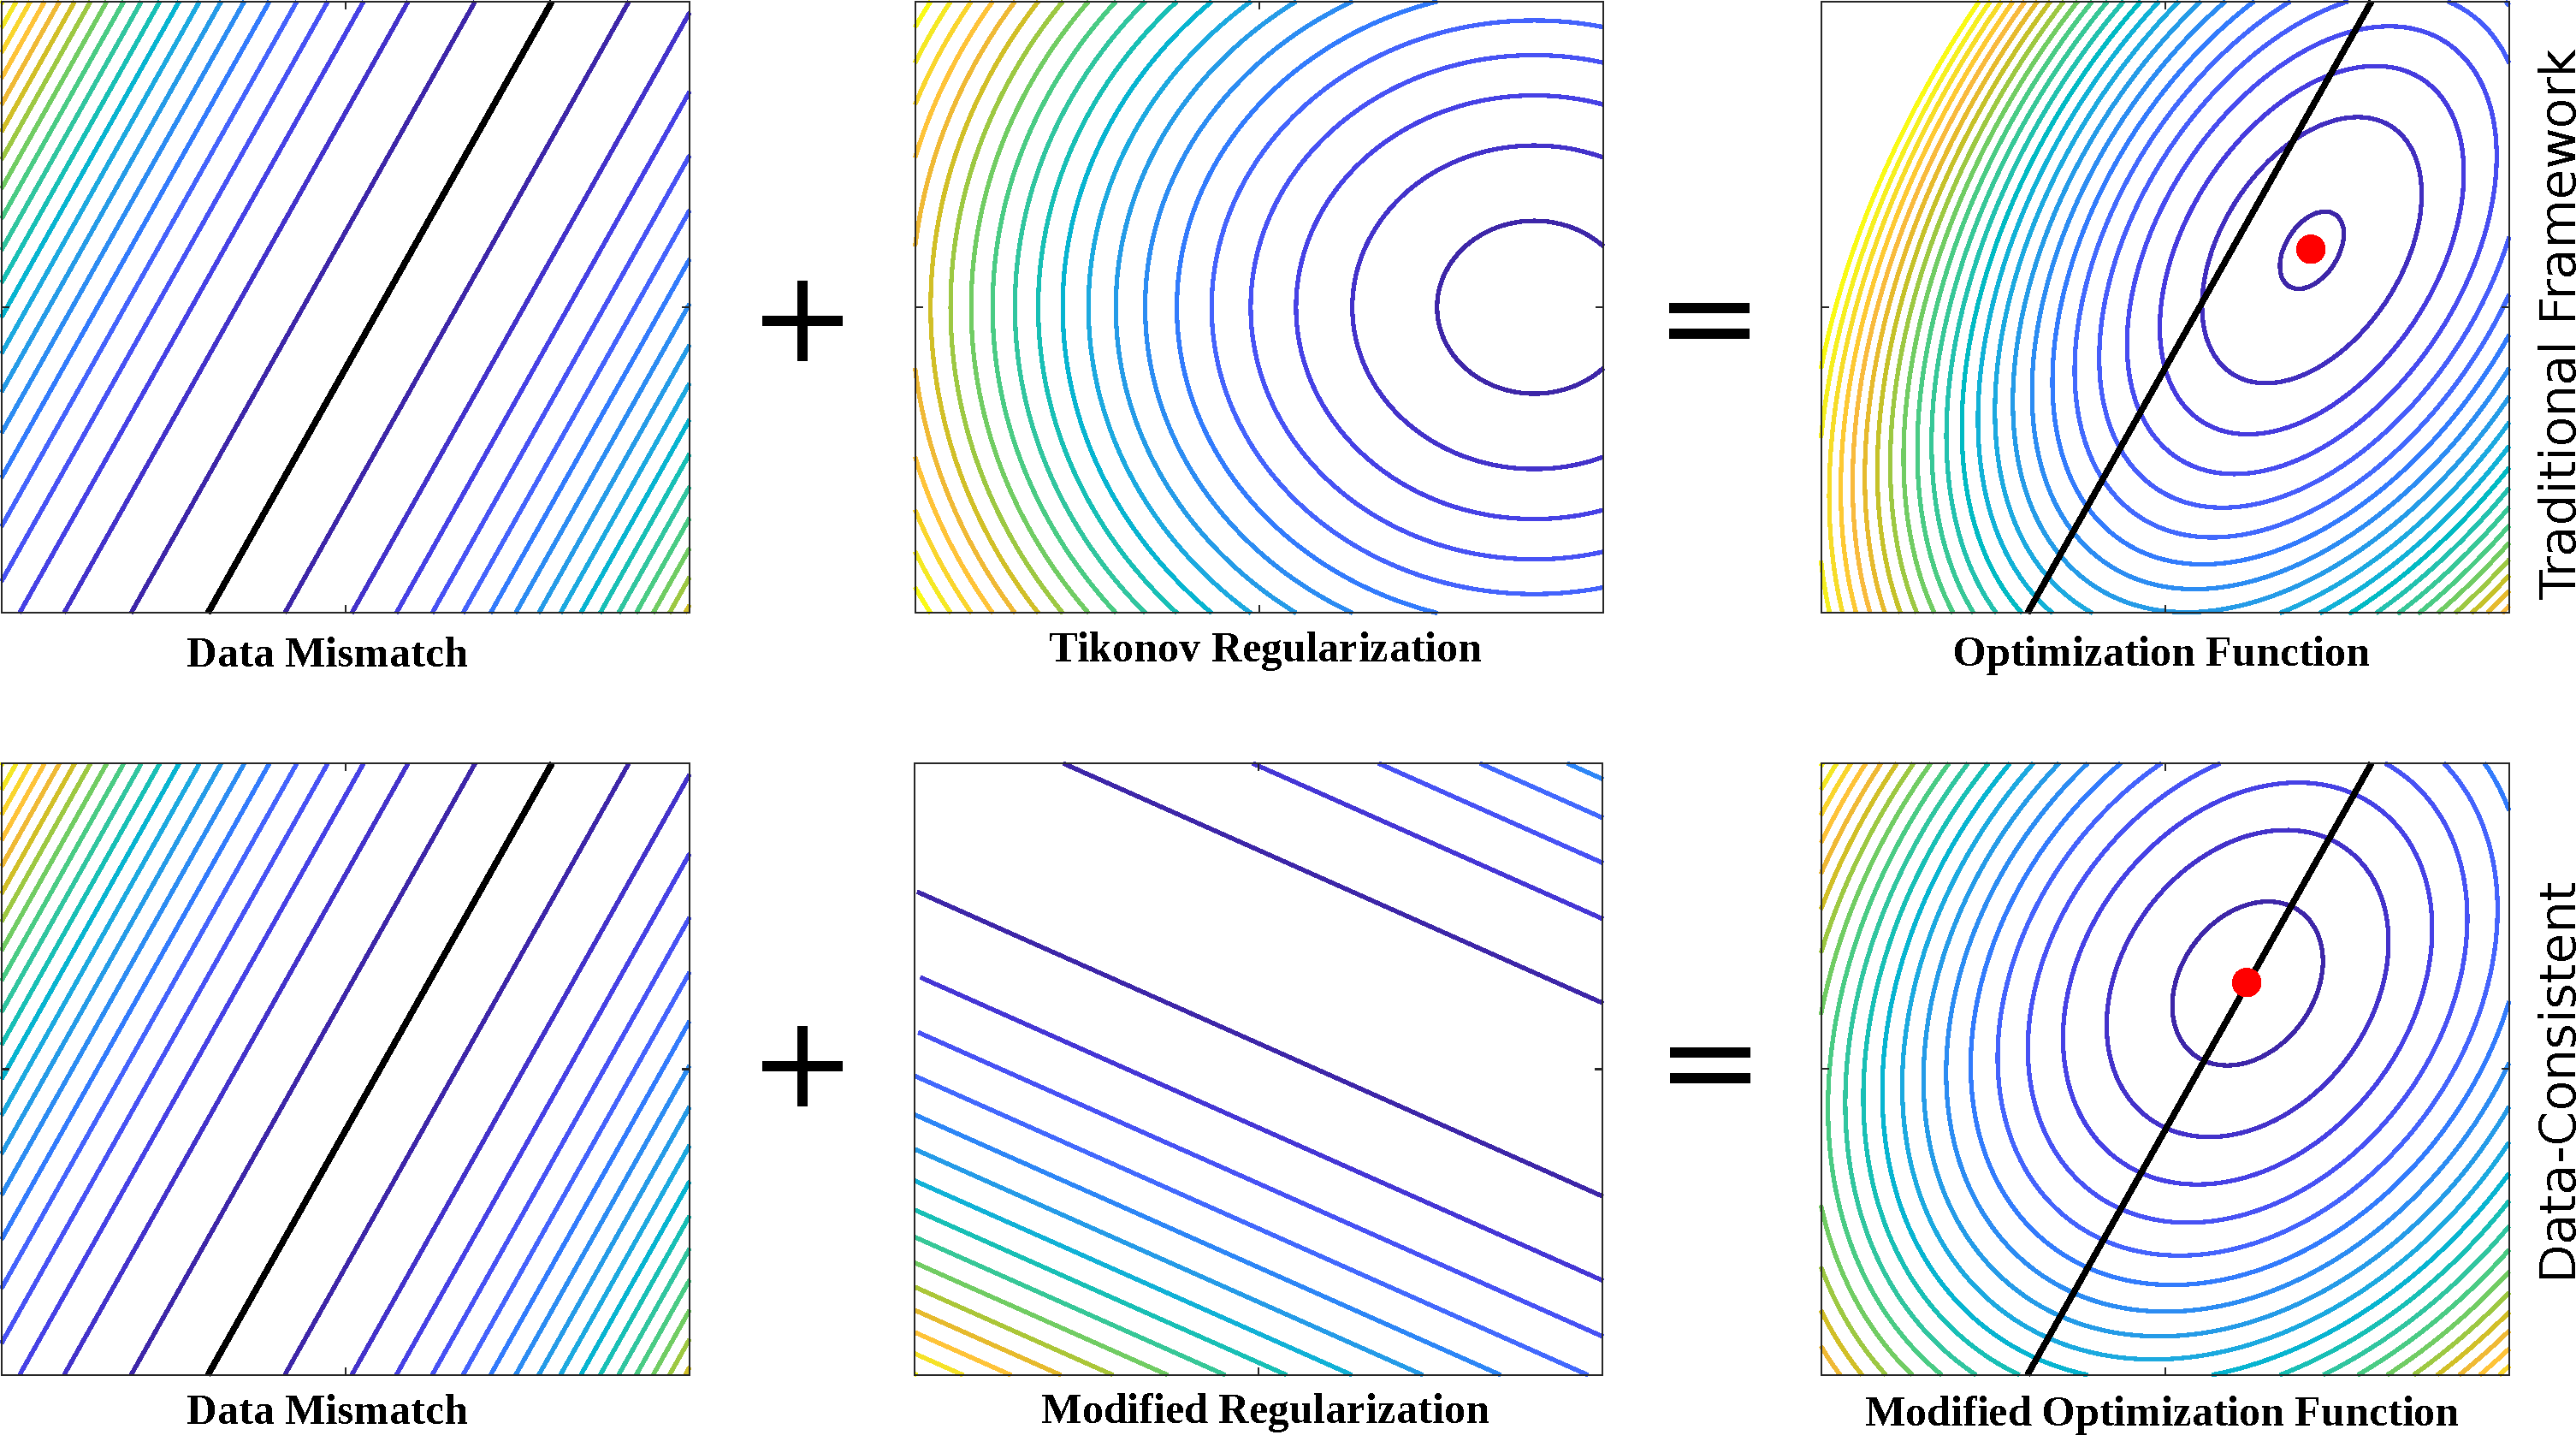
\includegraphics[width=\linewidth]{figures/Regularization-all-in-one.pdf}
  \centering
  \begin{tabular}{|ccc|}
    \hline
      \subf{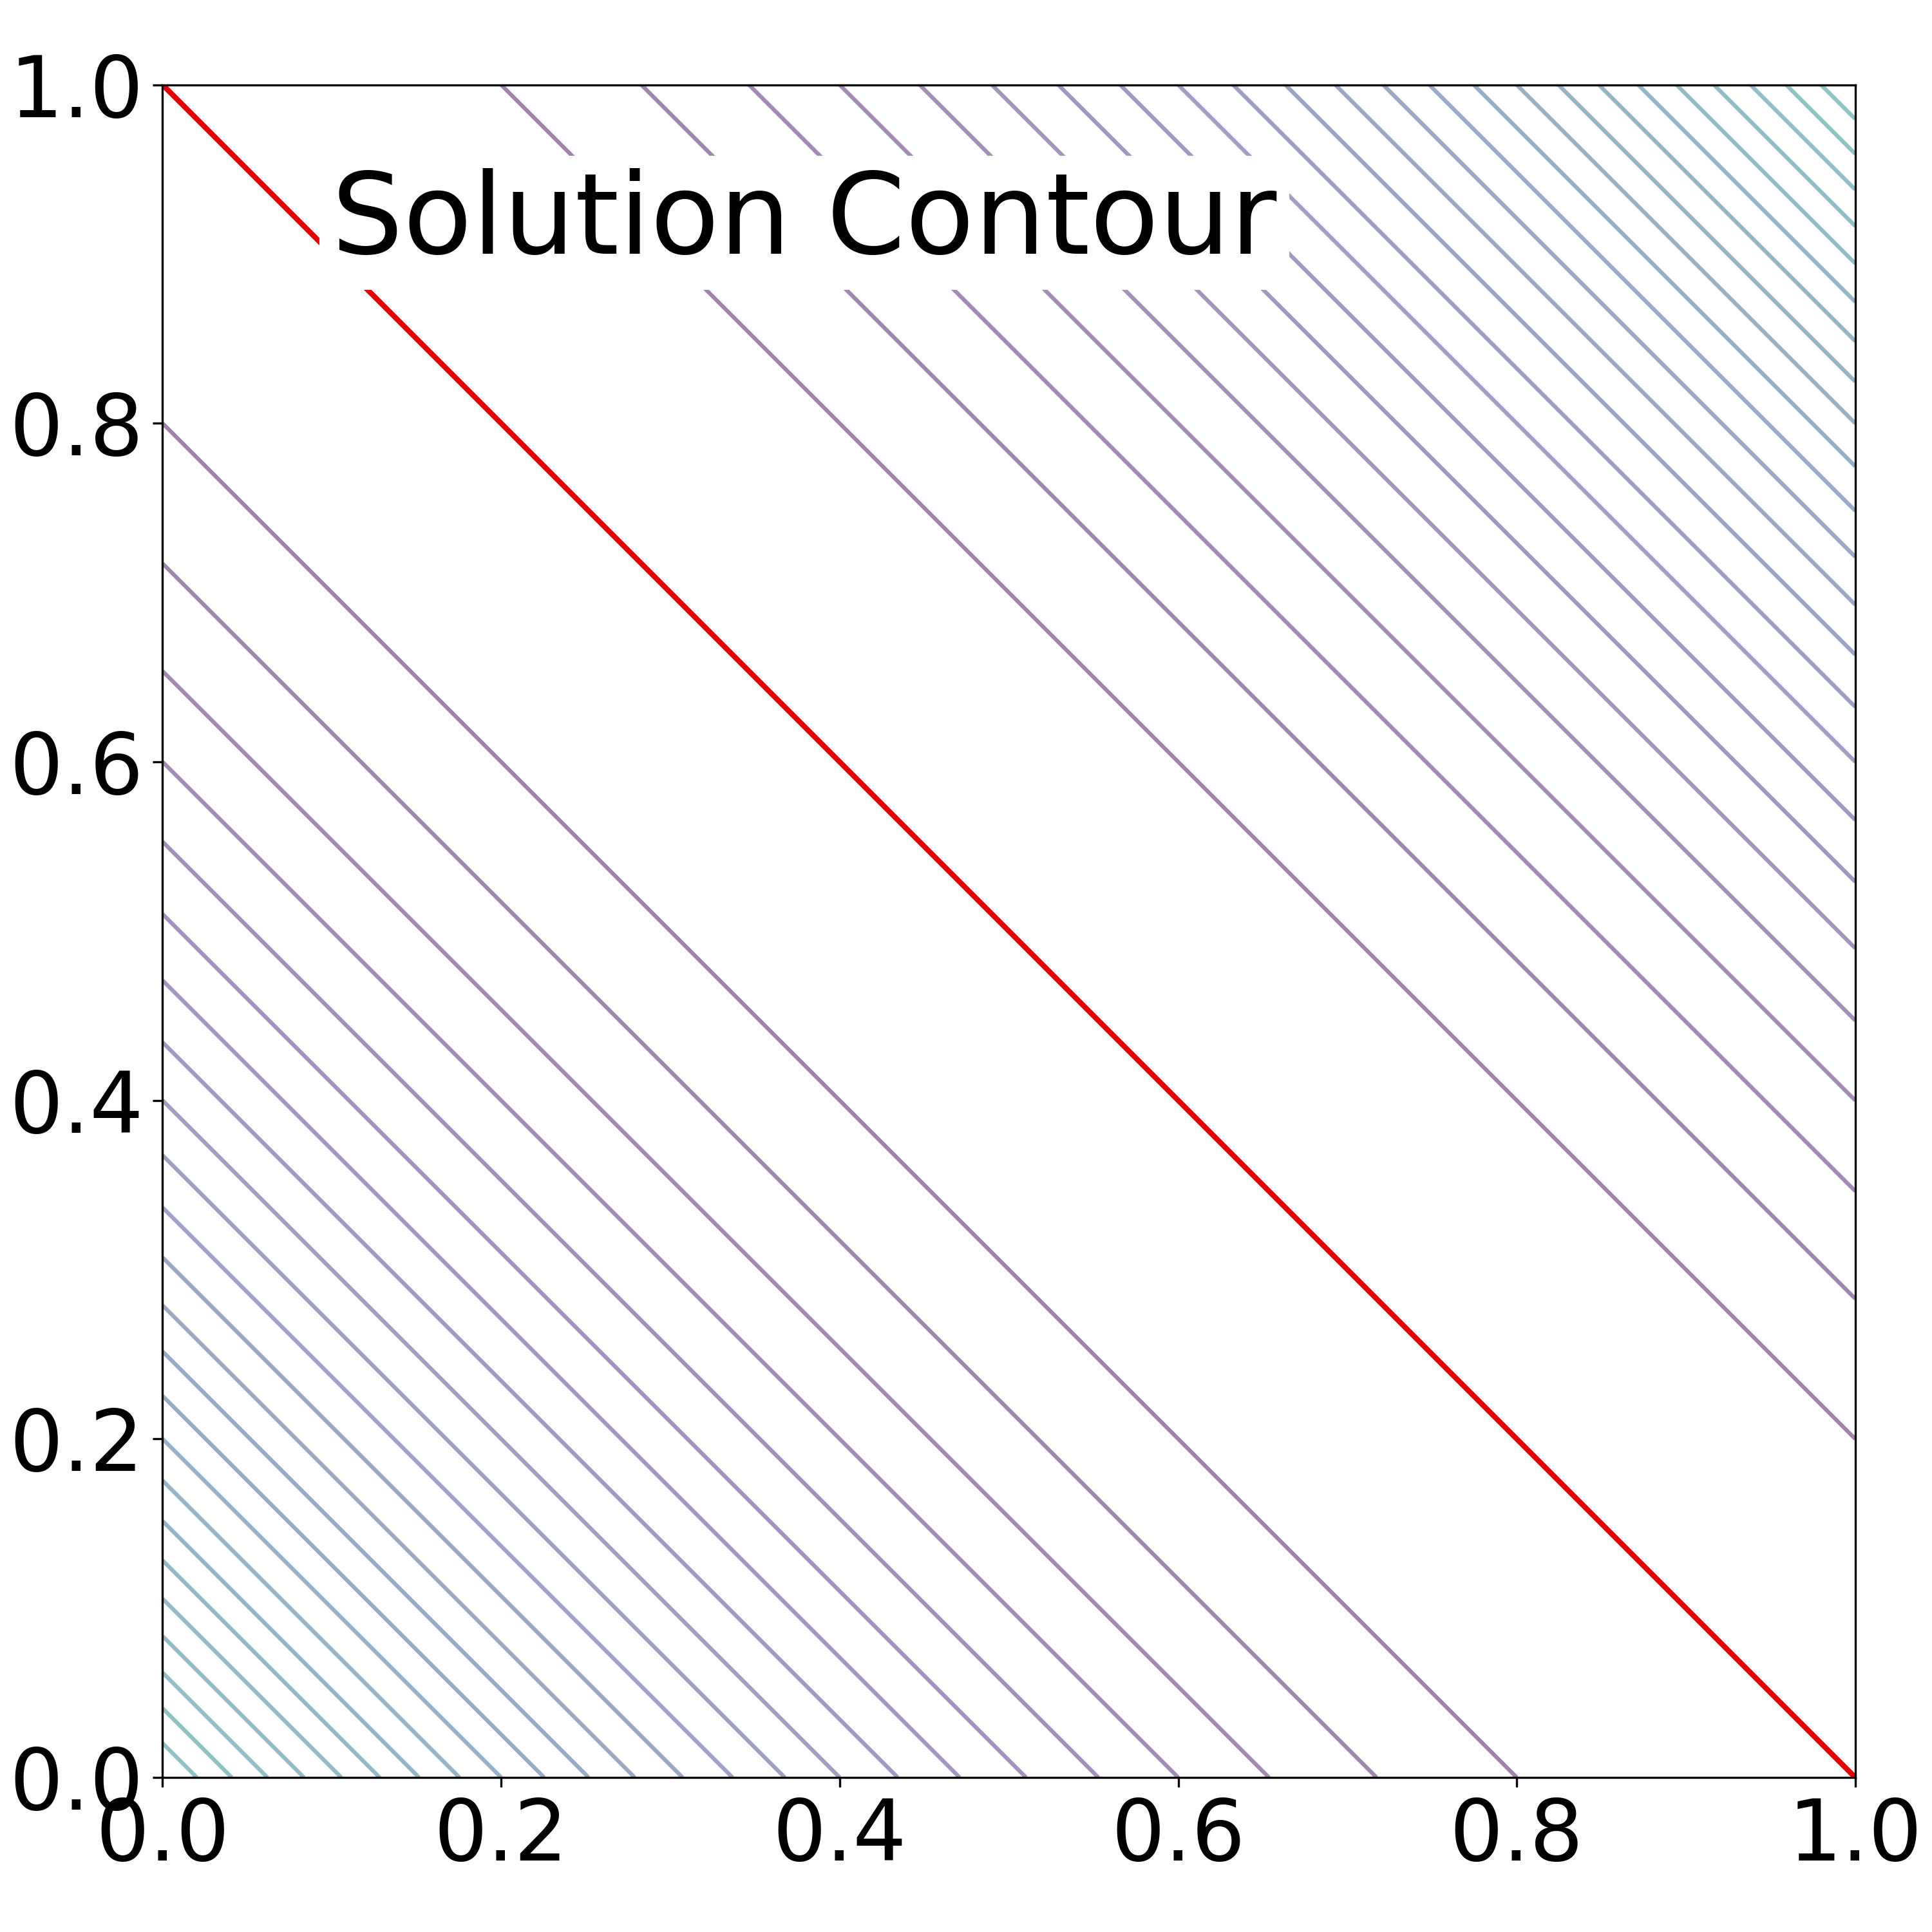
\includegraphics[width=0.25\linewidth]{figures/data_mismatch_contour.png}}
      {data mismatch}
    &
      \subf{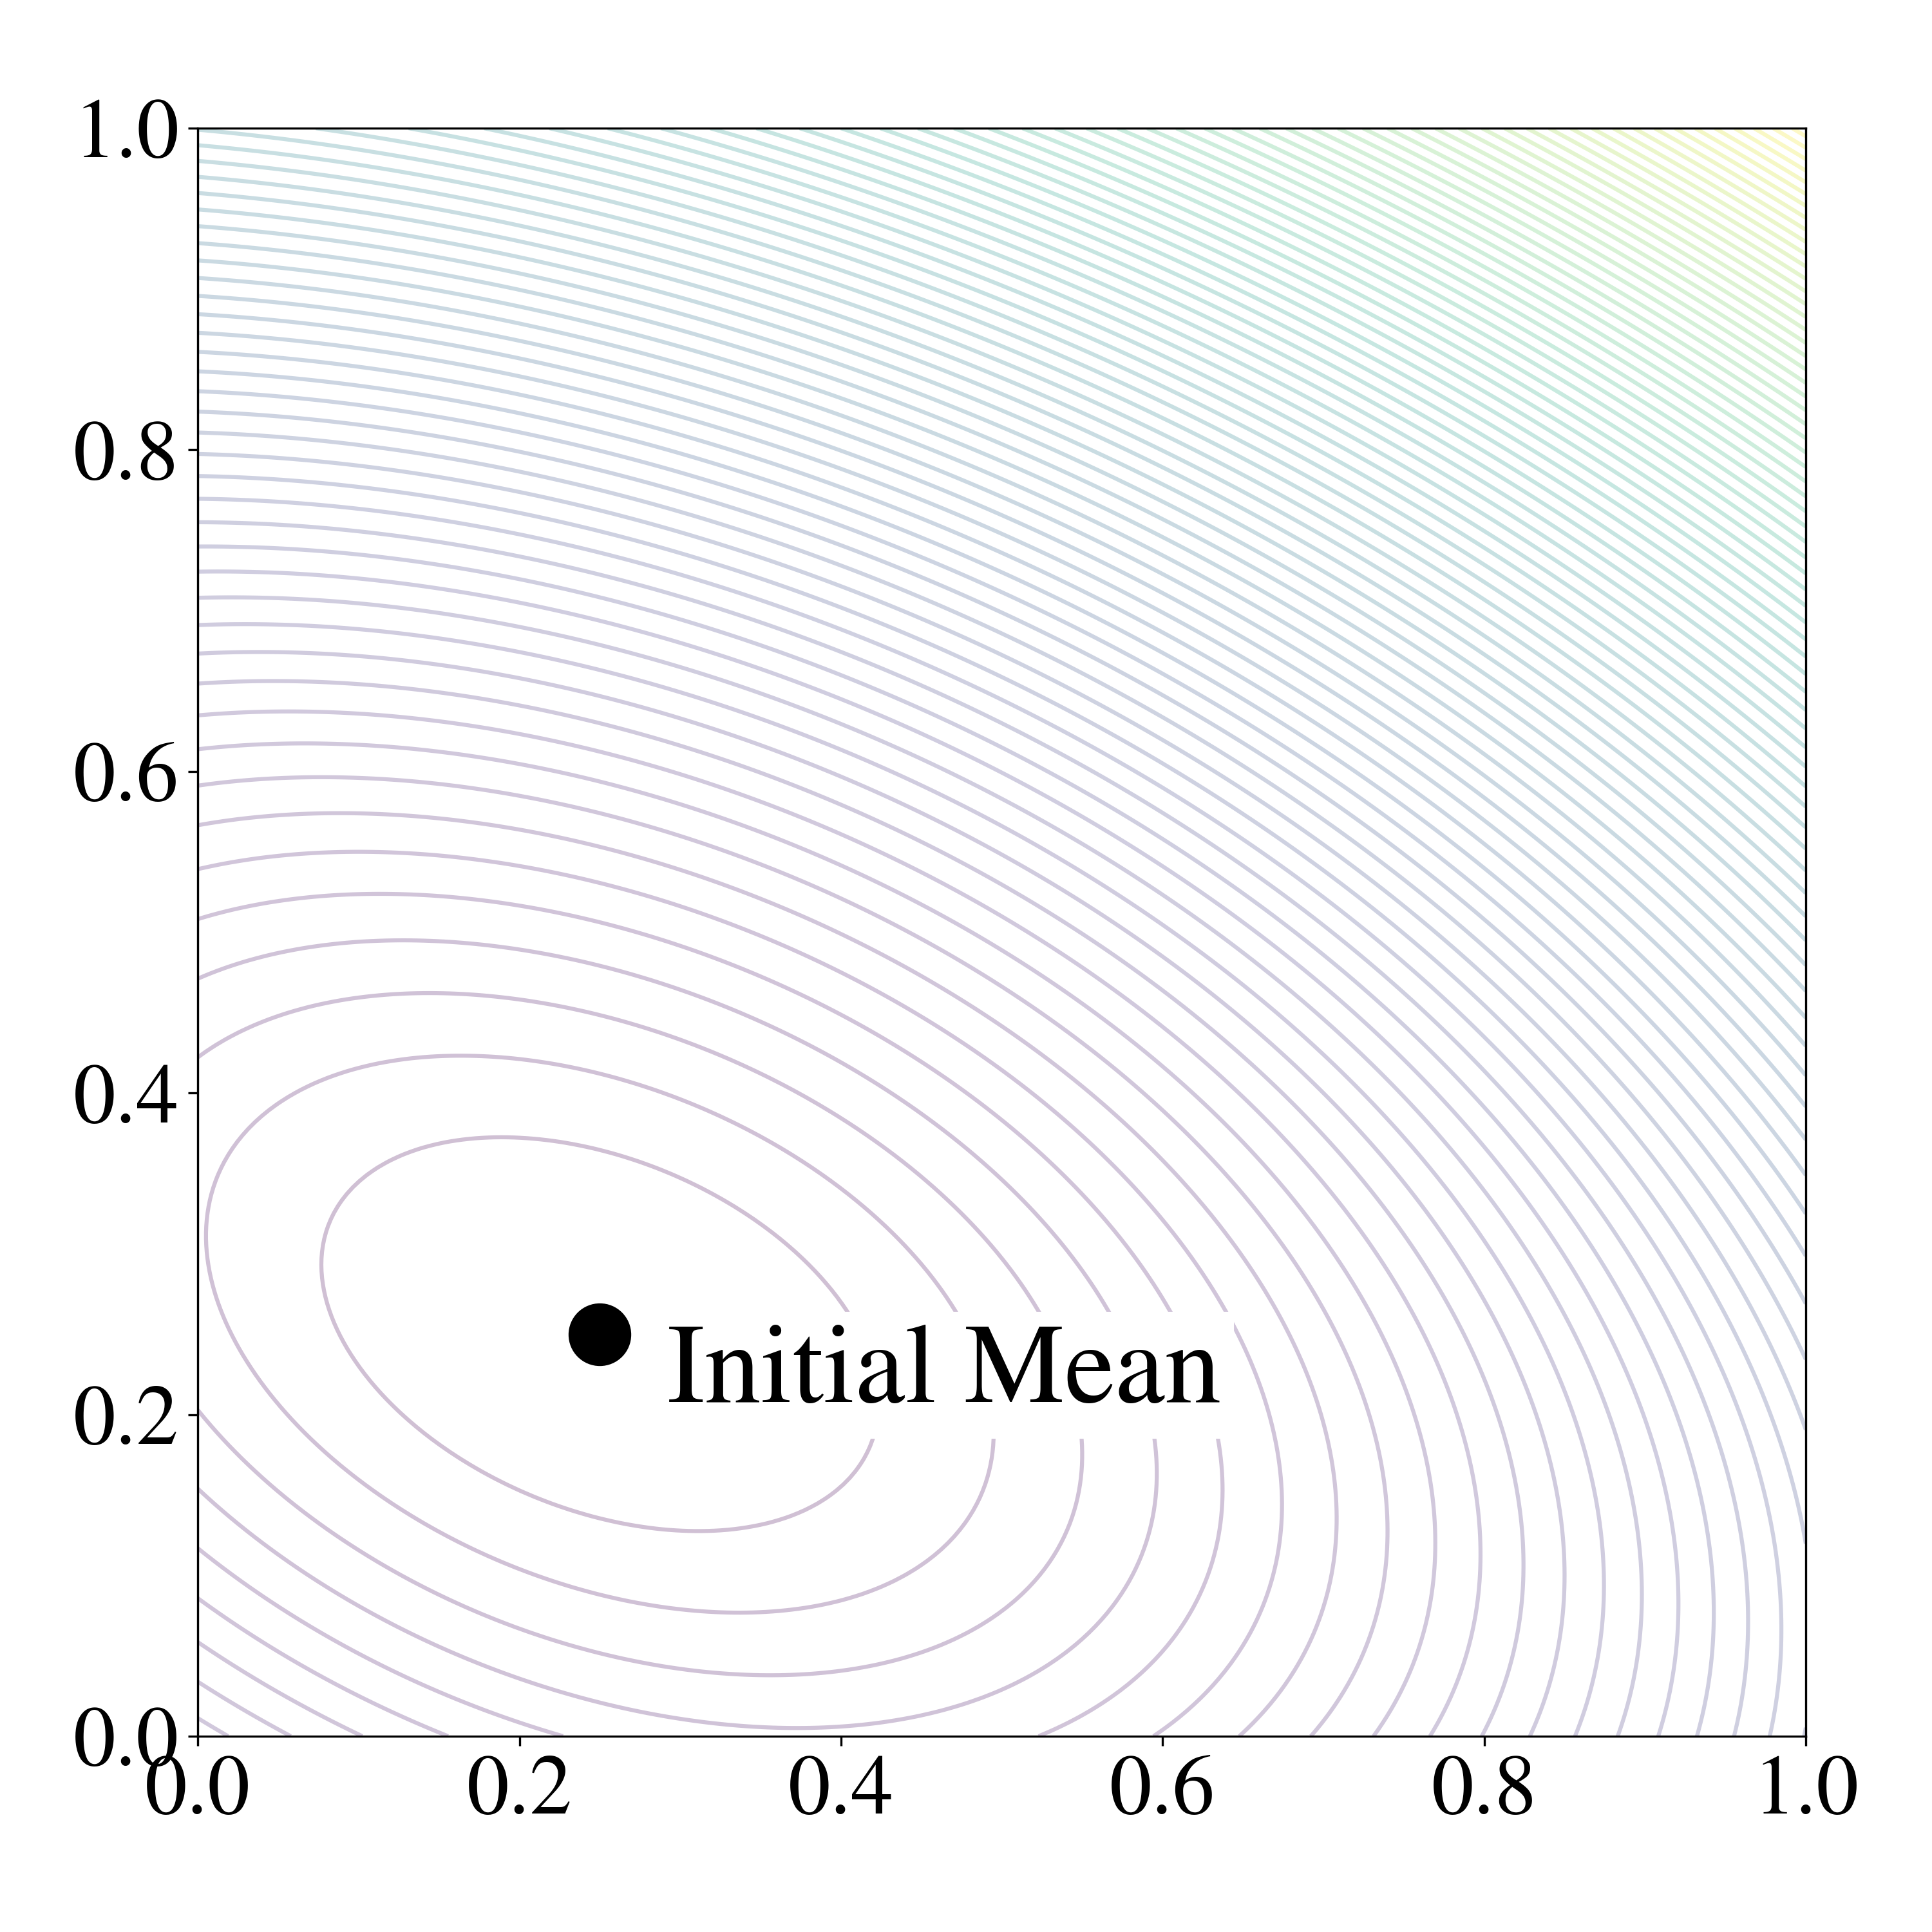
\includegraphics[width=0.25\linewidth]{figures/tikonov_contour.png}}
      {regularization}
    &
      \subf{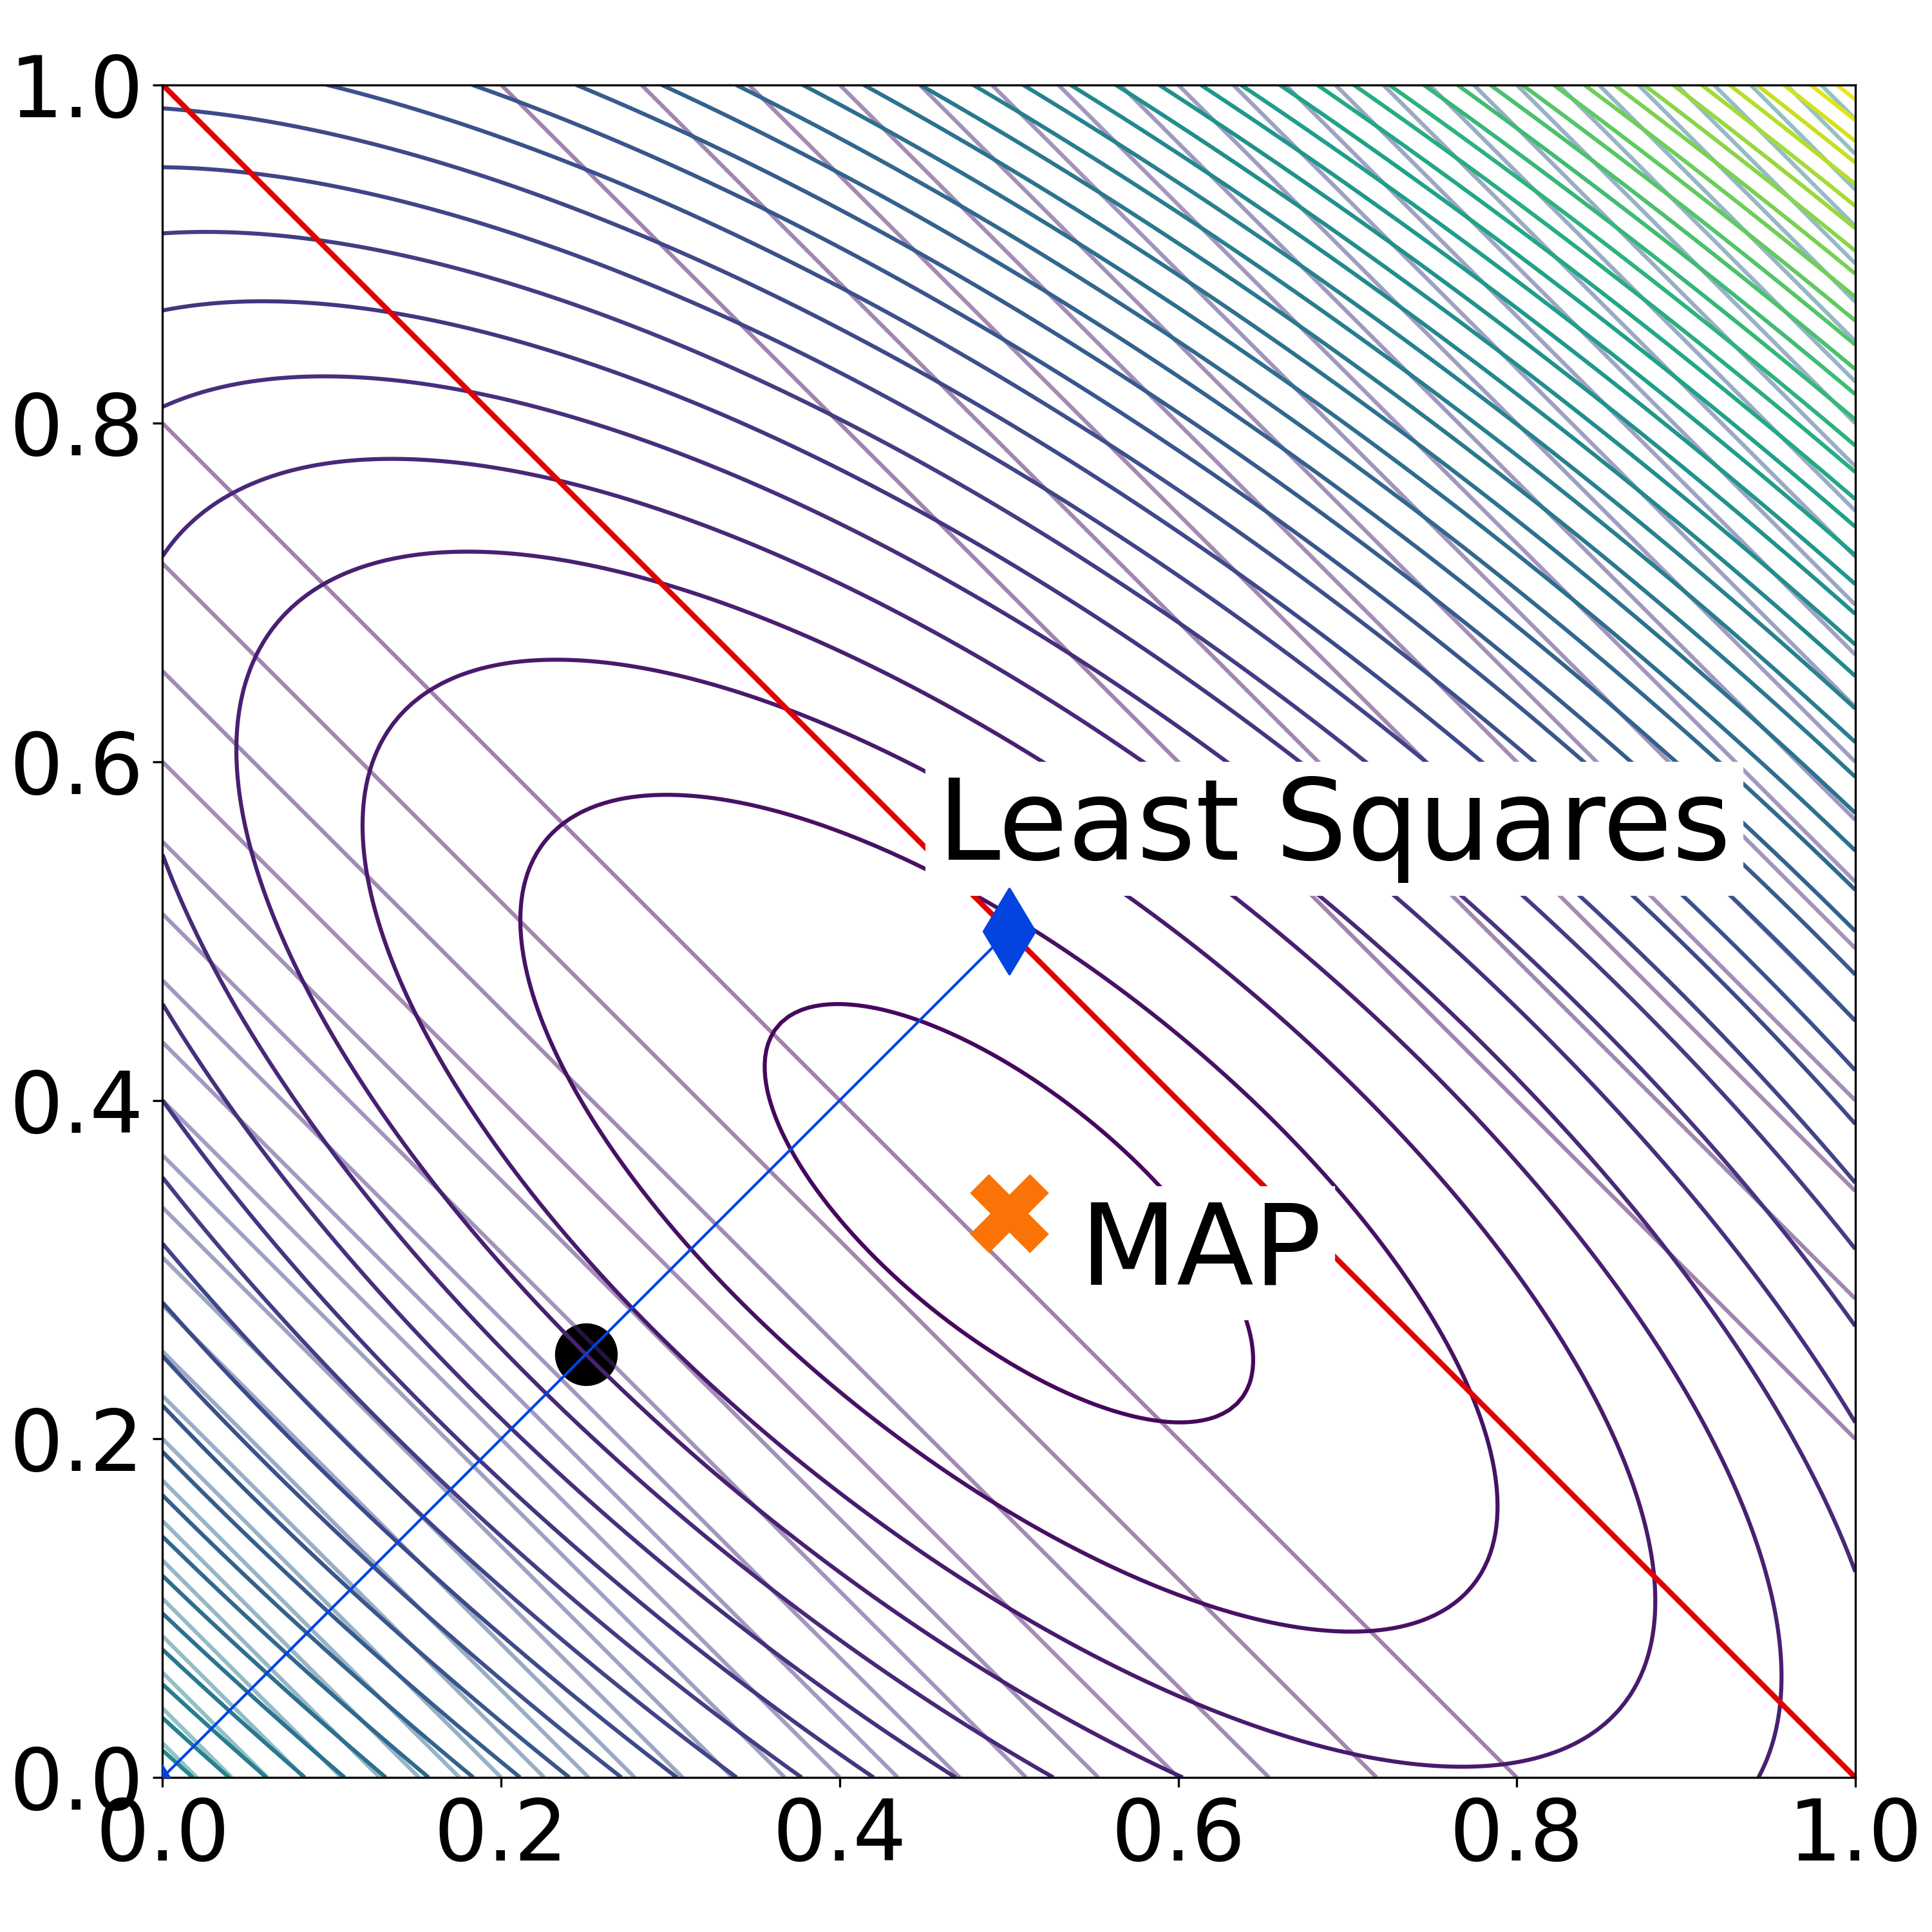
\includegraphics[width=0.25\linewidth]{figures/classical_solution.png}}
      {bayesian posterior}
    \\
    \hline
      \subf{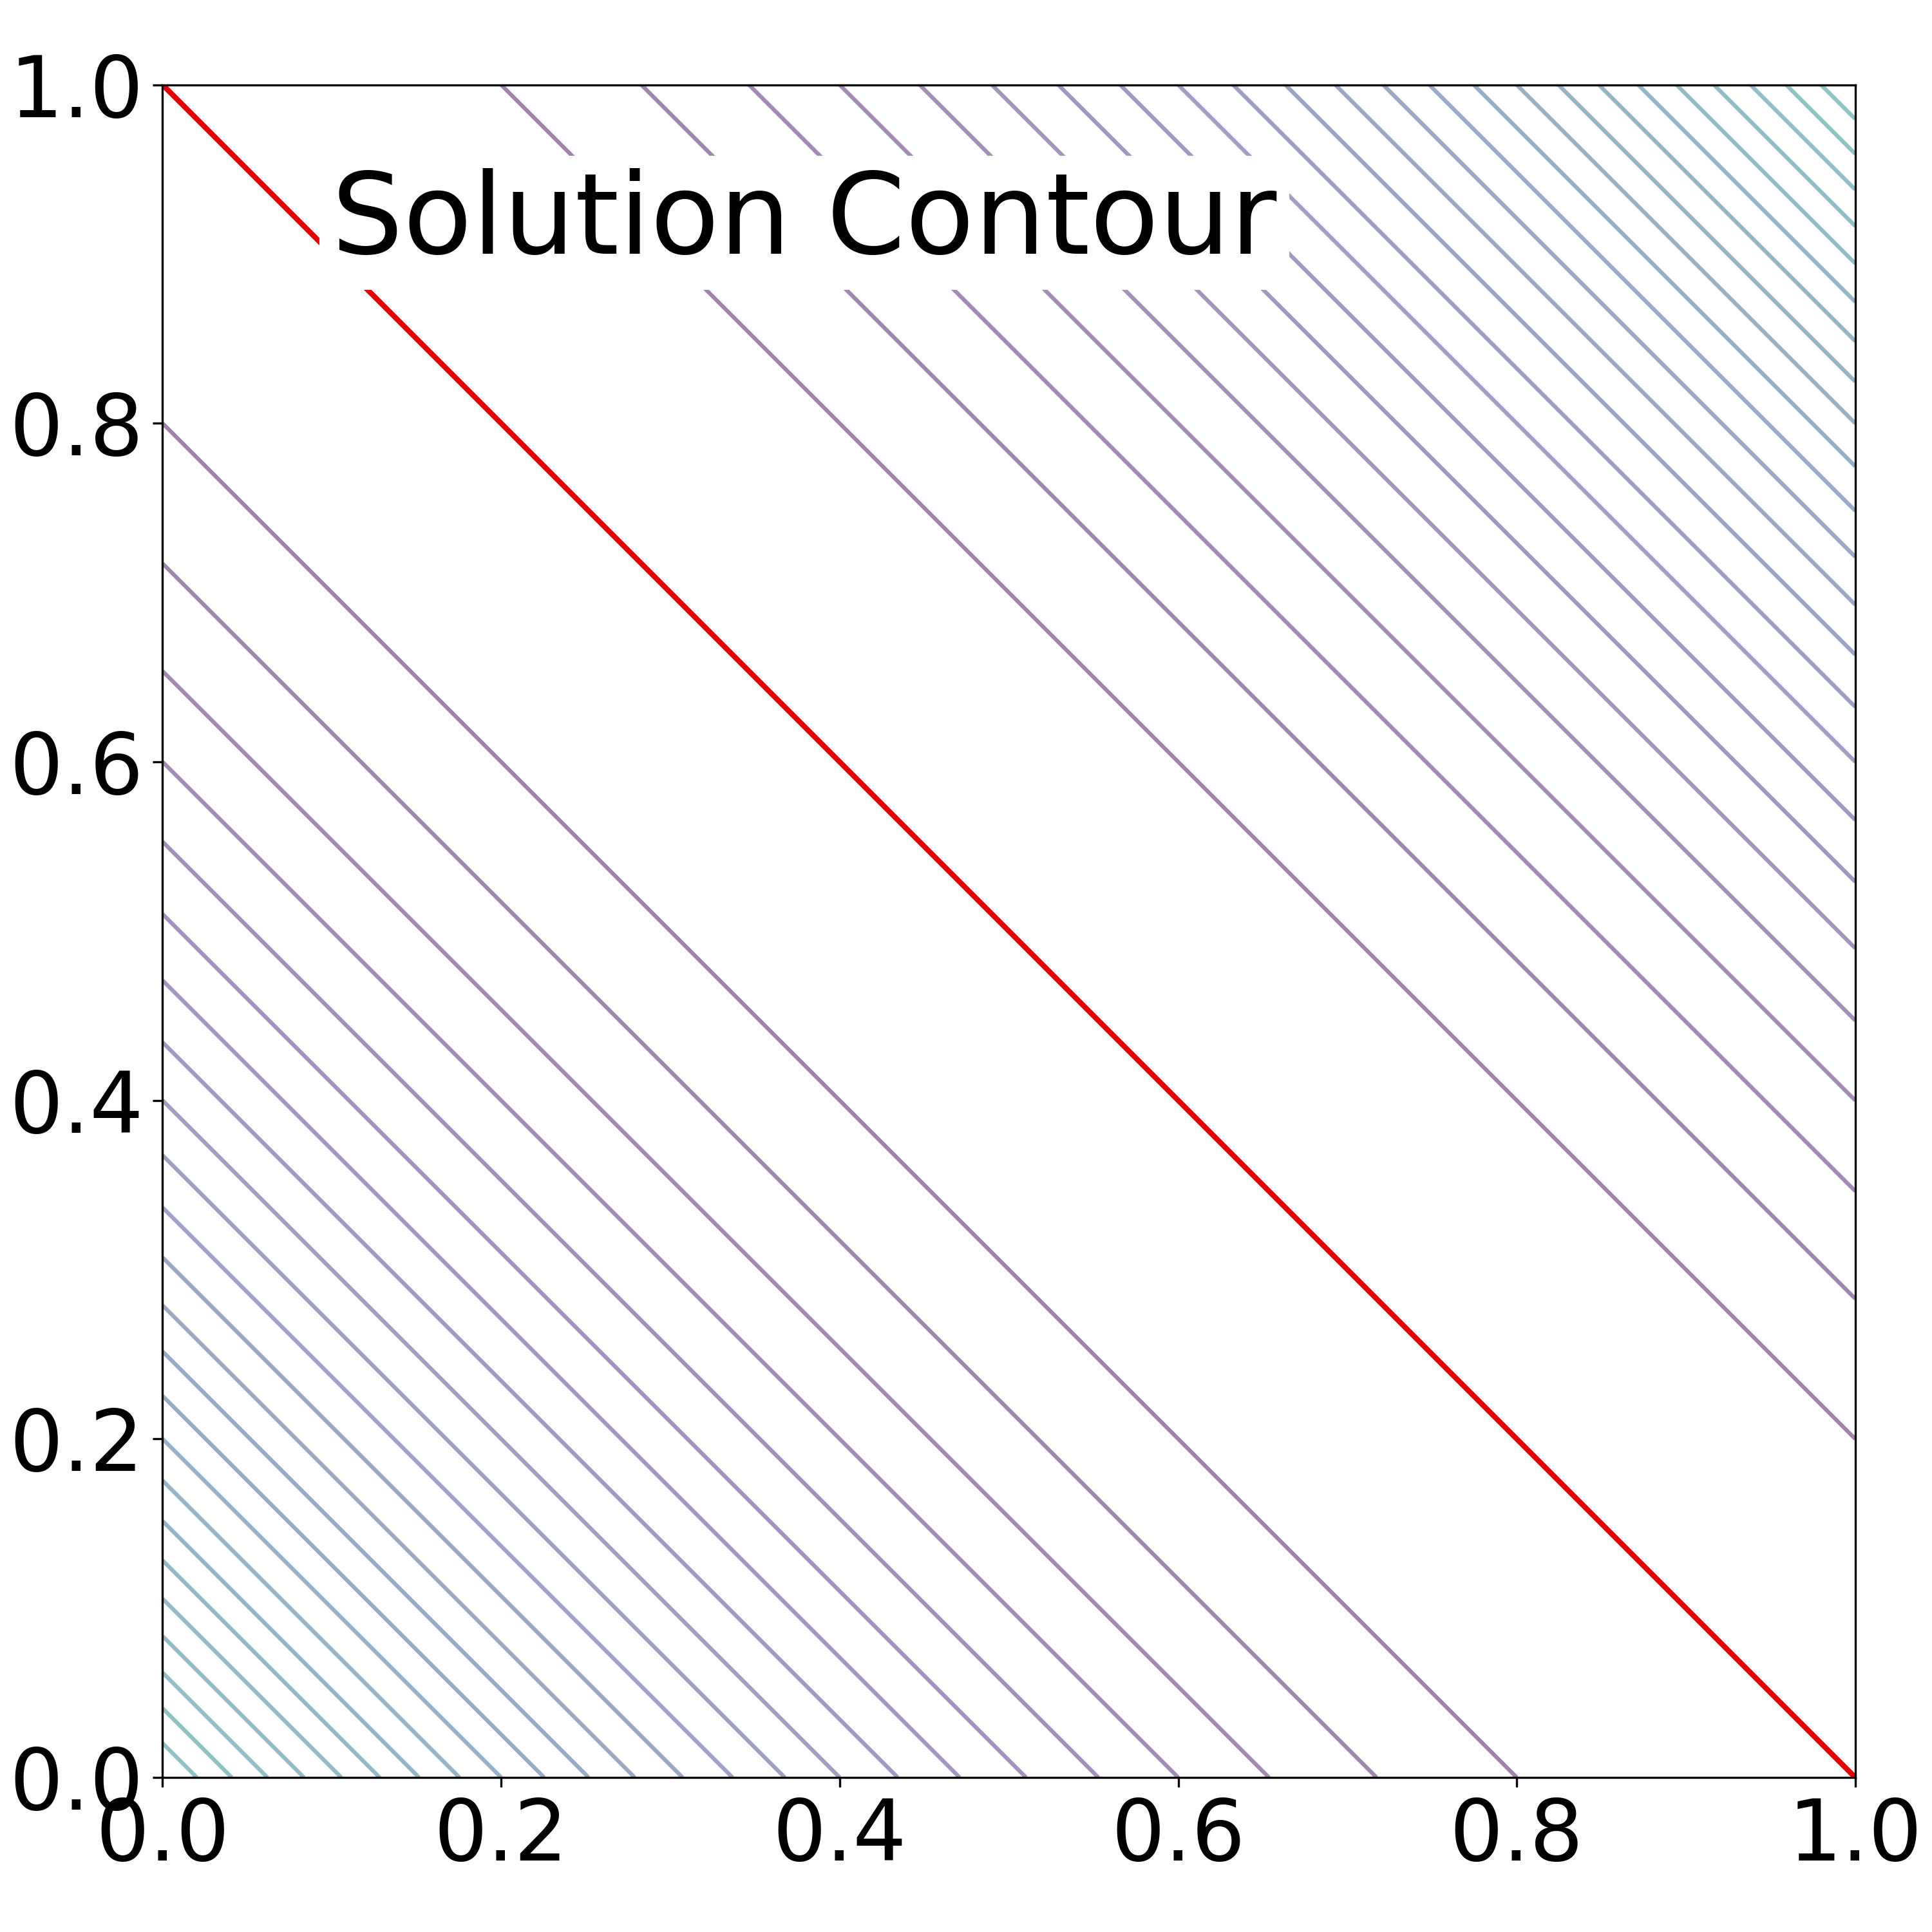
\includegraphics[width=0.25\linewidth]{figures/data_mismatch_contour.png}}
      {data mismatch}
    &
      \subf{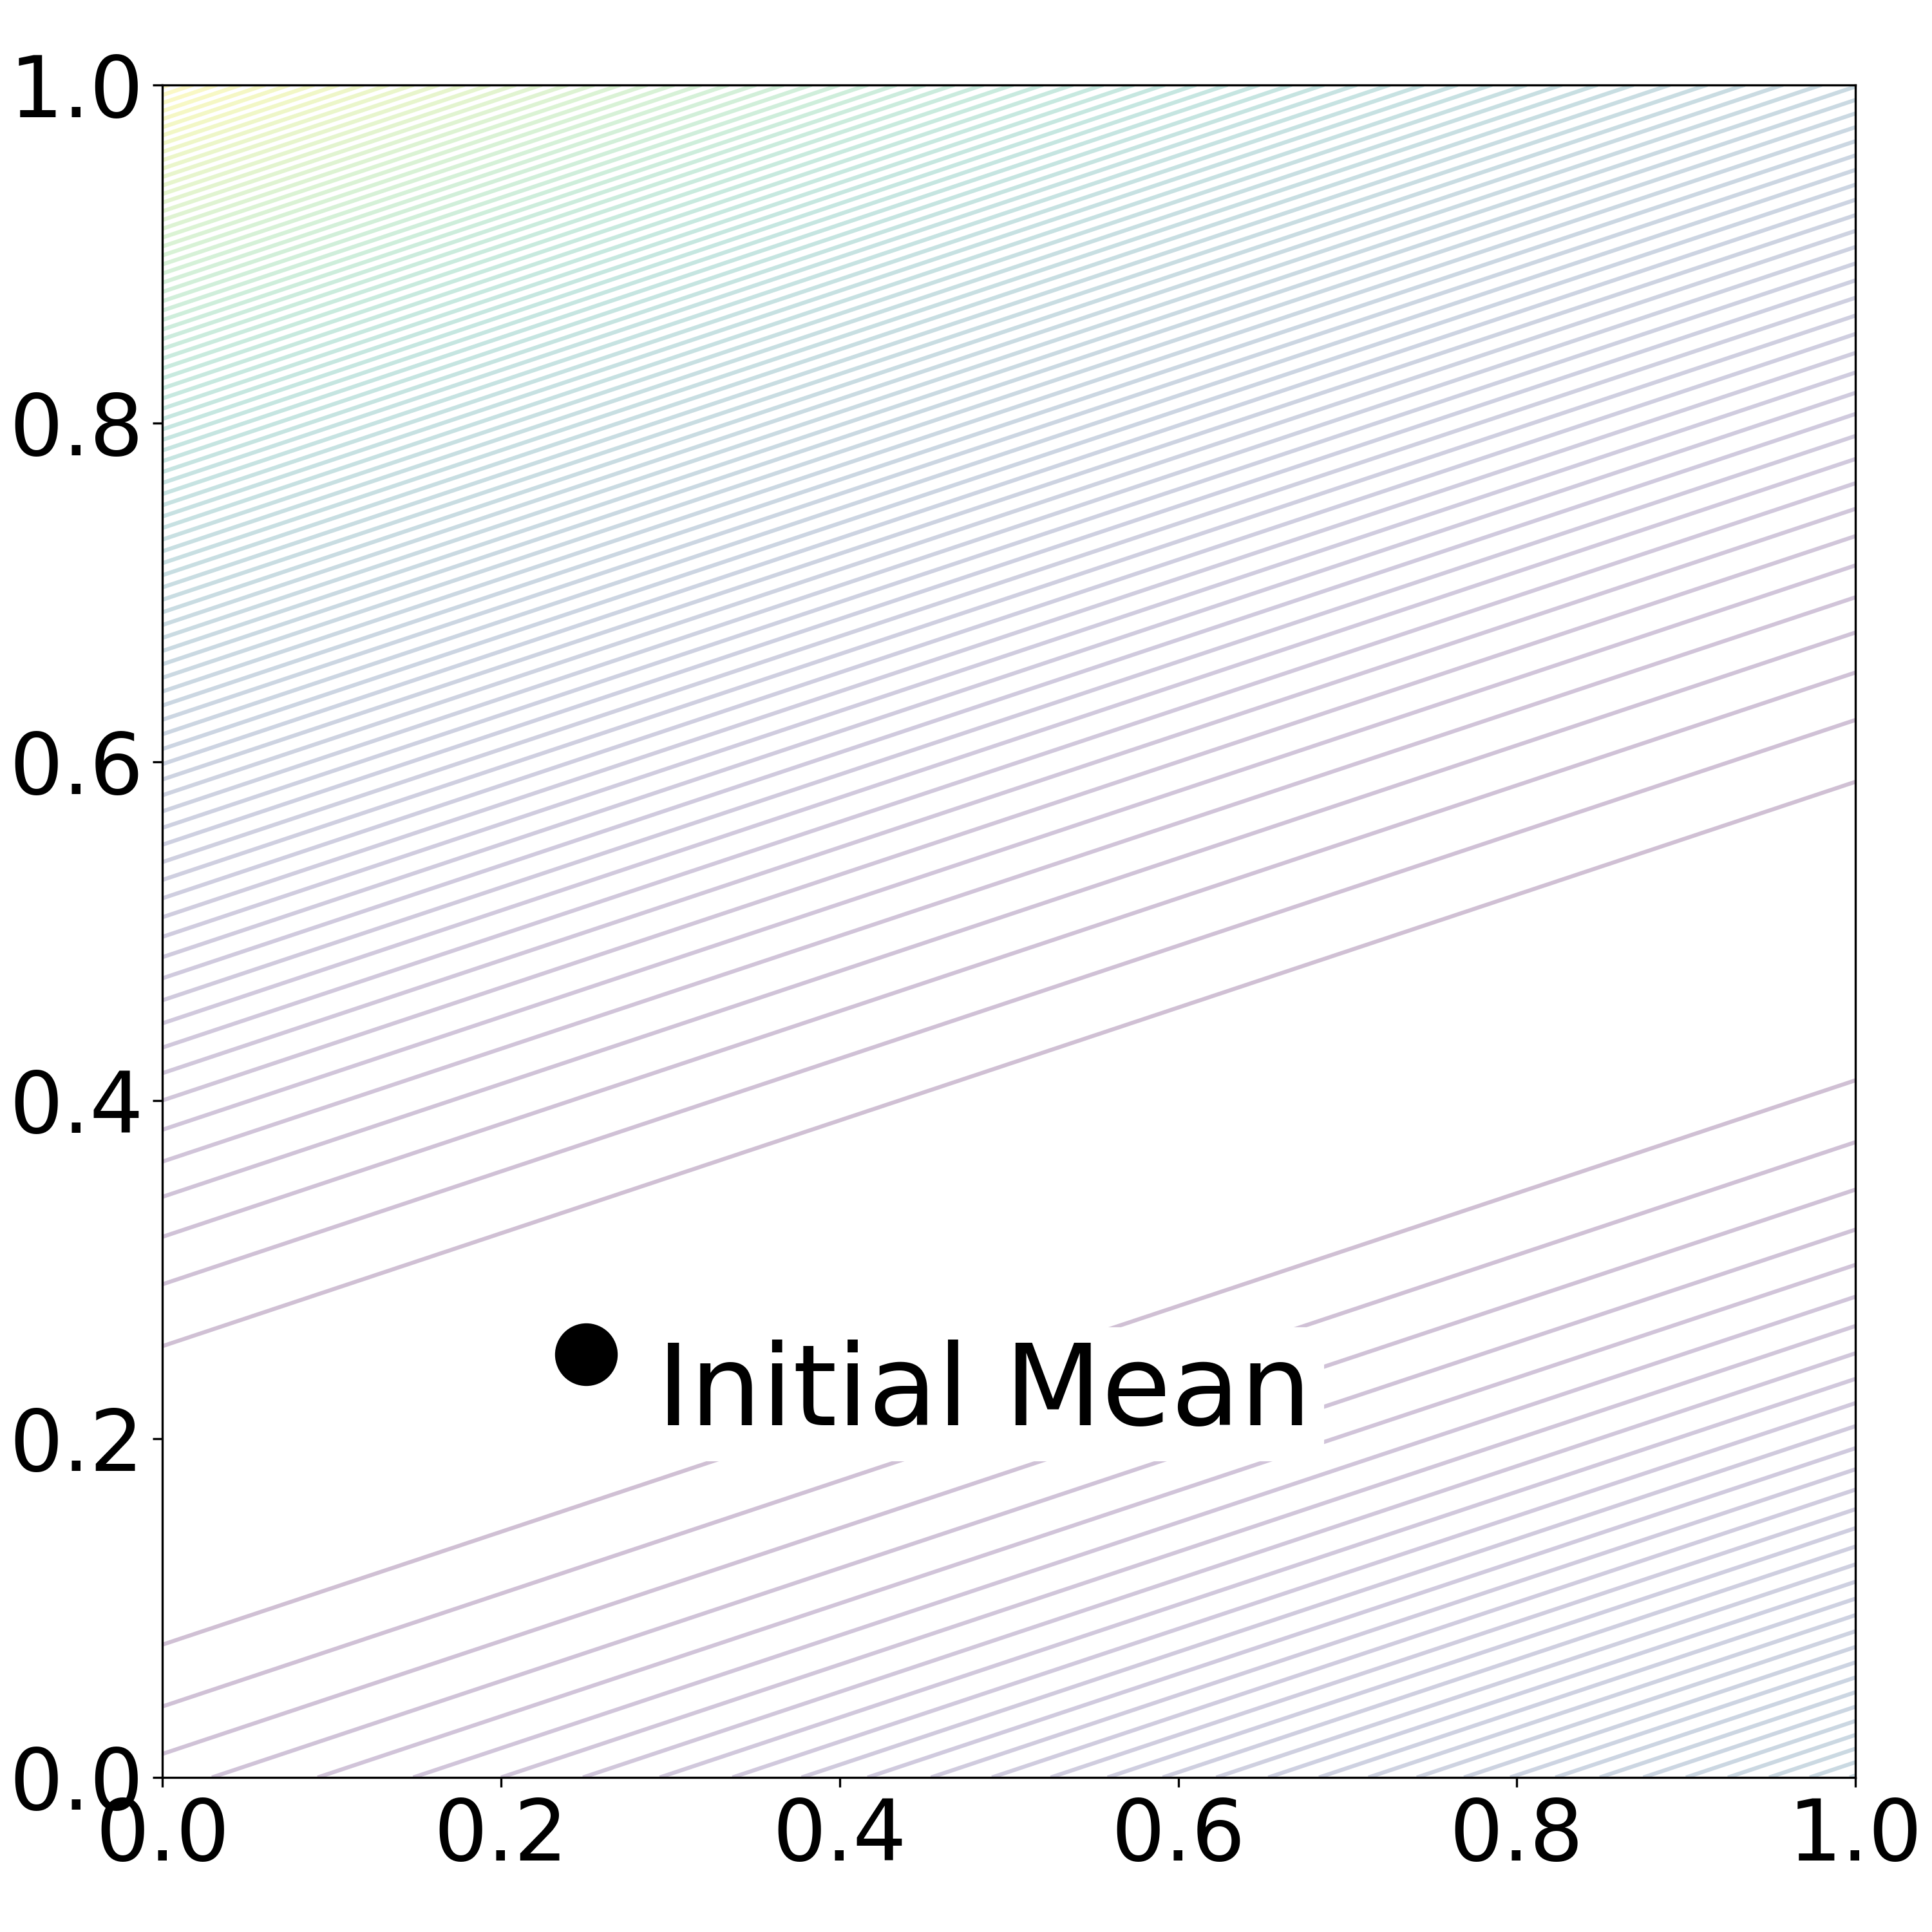
\includegraphics[width=0.25\linewidth]{figures/consistent_contour.png}}
      {modified regularization}
    &
      \subf{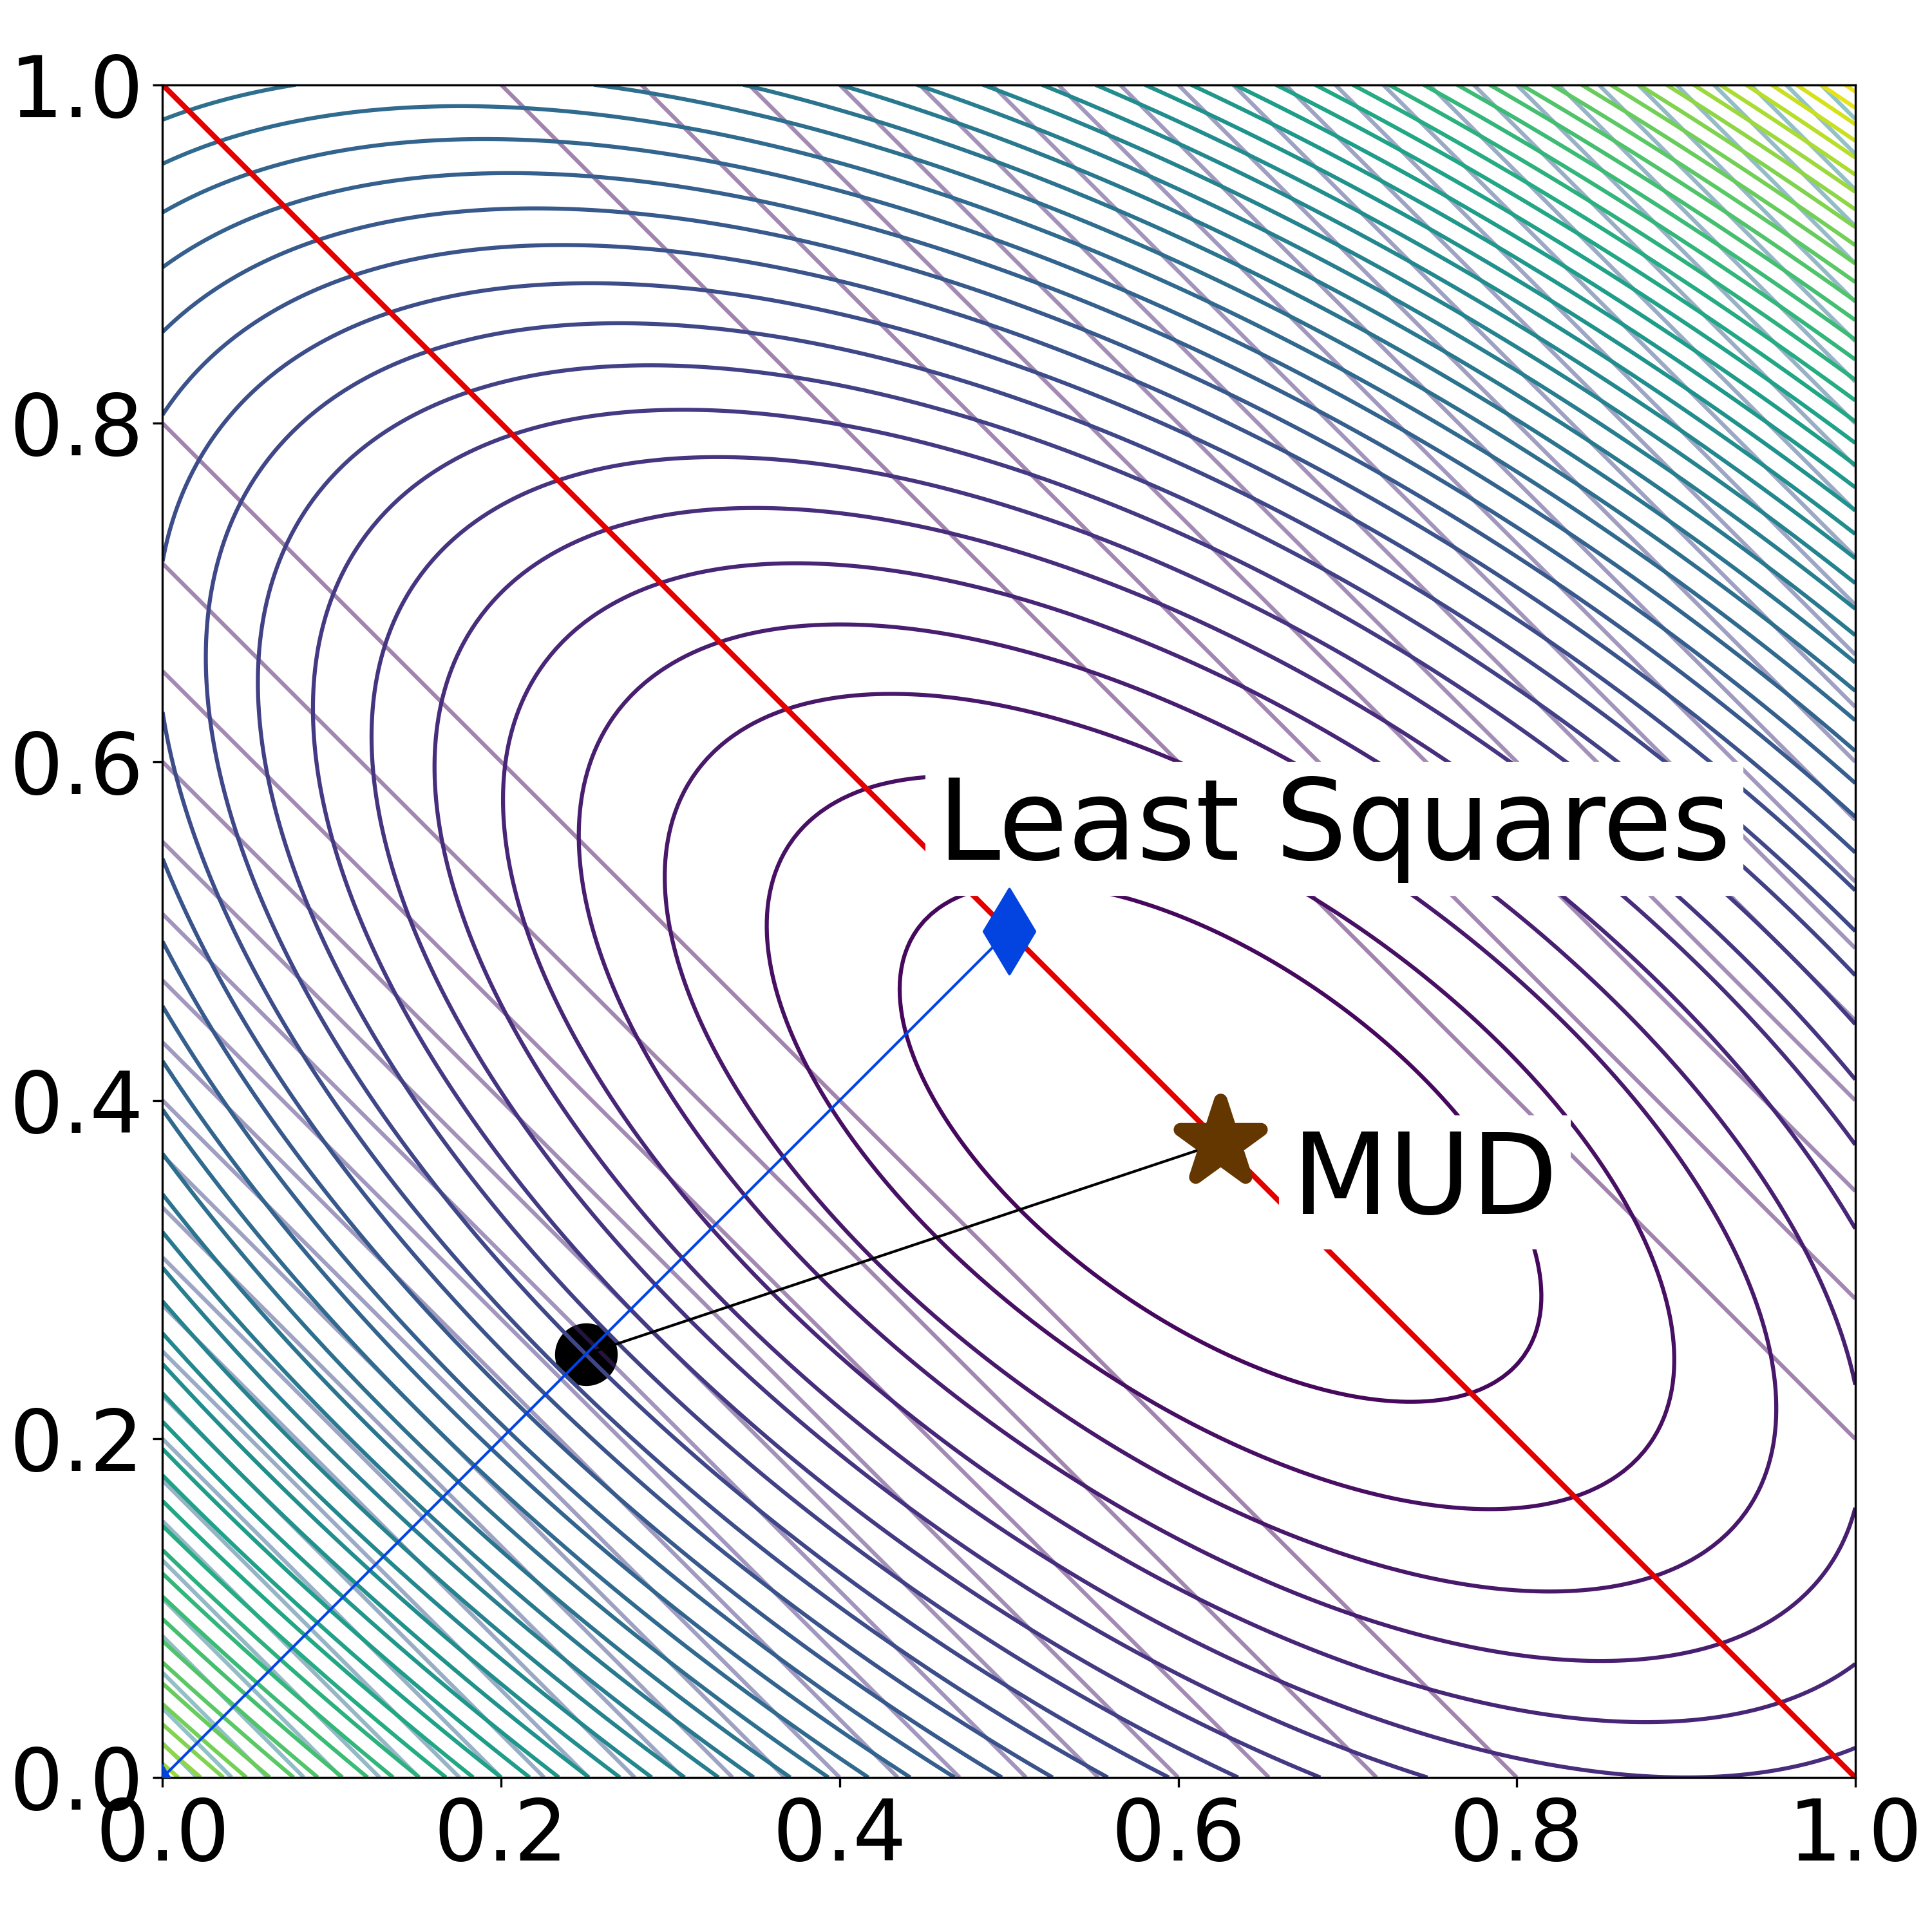
\includegraphics[width=0.25\linewidth]{figures/consistent_solution.png}}
       {updated density}
    \\
    \hline
  \end{tabular}

  \caption{Gaussian data mismatch for a 2-to-1 linear map (left plots). Gaussian initial/prior induce different regularization terms (middle plots), which leads to different optimization functions (right plots) and parameter estimates.}
  \label{fig:regularization}
\end{figure}


\end{figure}

\end{frame}


%%%%%%%%%%%%%%%%%%%%%%%%%%%%%%%%%%%%%%%%%%%%%%%%%%%%%%%%%%%
\subsection{Closed-Form Solutions}
%%%%%%%%%%%%%%%%%%%%%%%%%%%%%%%%%%%%%%%%%%%%%%%%%%%%%%%%%%%

\begin{frame}[t]
%\vskip 25pt
\centering

The posterior covariance is formally given by

\begin{equation}\label{eq:map_cov}
\Sigma_\text{post} := ( A^\top {\Sigma}_\text{obs}^{-1} A + \initialCov^{-1} )^{-1}.
\end{equation}

Applying Woodbury identity and~\eqref{eq:predictCov}, we rewrite the posterior covariance:

\begin{equation}\label{eq:map_cov_analytical}
\Sigma_\text{post} = \initialCov - \initialCov A^\top \left[\predictedCov + \observedCov\right]^{-1} A \initialCov
\end{equation}

Can now interpret $\Sigma_\text{post}$ as a rank $d$ correction (or update) of $\initialCov$. \\
$\predictedCov + \observedCov$ is invertible because it is the sum of two s.p.d matrices. \\
We rewrite the closed form expression for the MAP poing given in \cite{Tarantola_book} as

\begin{equation}\label{eq:map-point-analytical}
\param^{\text{MAP}} = \param_0 + \Sigma_\text{post} A^\top \observedCov^{-1} (\observedMean - b - A\param_0).
\end{equation}

\end{frame}


%%%%%%%%%%%%%%%%%%%%%%%%%%%%%%%%%%%%%%%%%%%%%%%%%%%%%%%%%%%
\begin{frame}[t]

We define
\begin{equation}\label{eq:eff_reg}
	R := \nolinebreak \initialCov^{-1} - \nolinebreak A^\top \predictedCov^{-1} A.
\end{equation}

Using this $R$, rewrite $J(\param)$ as

\begin{equation}\label{eq:dci-objective-alt}
J(\param):= \norm{\observedMean - Q(\param)}_{\observedCov^{-1}}^2 + \norm{\param - \param_0}_{R}^2.
\end{equation}

\vskip 12pt
In this form, we identify $R$ as the {\em effective regularization} in $J(\param)$ due to the formulation in the data-consistent framework.
\begin{equation}
	\updatedCov := \left(A^\top \observedCov^{-1} A + R\right)^{-1}.
\end{equation}

Since $R$ is not invertible, Woodbury's identity cannot be applied (yet).
\end{frame}

%%%%%%%%%%%%%%%%%%%%%%%%%%%%%%%%%%%%%%%%%%%%%%%%%%%%%%%%%%%
\begin{frame}[t]
%\vskip 25pt
\centering
We derive using several identities
\begin{equation}\label{eq:updatedCov_final}
	\updatedCov = \initialCov - \initialCov A^\top \predictedCov^{-1}\left[\predictedCov-\observedCov\right]\predictedCov^{-1}A\initialCov.
\end{equation}

\vskip 12pt
Substitute $\updatedCov$ for $\Sigma_\text{post}$ in \eqref{eq:map-point-analytical} to write the point that minimizes $J$ as:

\begin{equation}\label{eq:mud-point-analytical-alt}
\param^{\text{MUD}} = \param_0 + \updatedCov A^\top \observedCov^{-1} (\observedMean - b - A\param_0).
\end{equation}

\vskip 12pt
Substituting~\eqref{eq:updatedCov_final} into~\eqref{eq:mud-point-analytical-alt} and simplifying, we have
\begin{equation}\label{eq:mud-point-analytical-final}
	\mudpt = \param_0 + \initialCov A^\top \predictedCov^{-1}(\observedMean - b - A\param_0).
\end{equation}

\end{frame}


%%%%%%%%%%%%%%%%%%%%%%%%%%%%%%%%%%%%%%%%%%%%%%%%%%%%%%%%%%%
\subsection{Impact of Information Content}
%%%%%%%%%%%%%%%%%%%%%%%%%%%%%%%%%%%%%%%%%%%%%%%%%%%%%%%%%%%

\begin{frame}[t]
%\vskip 25pt
\centering
\begin{figure}
\centering

The one where we show how rank and dimension impact our solutions.

\end{figure}

\end{frame}


%%%%%%%%%%%%%%%%%%%%%%%%%%%%%%%%%%%%%%%%%%%%%%%%%%%%%%%%%%%
\subsection{Data-Driven QoI Maps}
%%%%%%%%%%%%%%%%%%%%%%%%%%%%%%%%%%%%%%%%%%%%%%%%%%%%%%%%%%%

\begin{frame}[t]
%\vskip 25pt
\centering
\begin{figure}
\centering

The one where we show how to leverage this framework for general streams of data.

\end{figure}

\end{frame}


%%%%%%%%%%%%%%%%%%%%%%%%%%%%%%%%%%%%%%%%%%%%%%%%%%%%%%%%%%%
\subsection{Nonlinear Examples}
%%%%%%%%%%%%%%%%%%%%%%%%%%%%%%%%%%%%%%%%%%%%%%%%%%%%%%%%%%%

\begin{frame}[t]
%\vskip 25pt
\centering
\begin{figure}
\centering

The one where we show that our approach works even when some assumptions are violated.

\end{figure}

\end{frame}
